% Relatório da versão 1 do software ipump para o curso
% Sistemas de Controle - DCA0206 - UFRN
% Autores:
%   AUGUSTO MATHEUS PINHEIRO DAMASCENO
%   MARCEL DA CÂMARA RIBEIRO DANTAS
%   PABLO HOLANDA CARDOSO
%   PEDRO DE CASTRO GURGEL LIMA
%   RODRIGO DANTAS DA SILVA
% Modificado por: Ícaro Bezerra Queiroz de Araújo
%

%%%%%%%%%%%% STRUCTURE %%%%%%%%%%%%%%%
\documentclass[a4paper,12pt]{article}
\usepackage[T1]{fontenc}
\usepackage[utf8]{inputenc}
\usepackage[brazil]{babel}
\usepackage{lmodern}
\usepackage{setspace}
\usepackage[top=2cm, bottom=2cm, left=2cm, right=2cm]{geometry}
%%%%%%%%%%%%%%%%%%%%%%%%%%%%%%%%%%%%%%

%%%%%%%%%%%%%%%% PAGES STYLE %%%%%%%%%
\usepackage{fancyhdr}
\fancypagestyle{main}{
\renewcommand{\headrulewidth}{0pt}
\fancyhead[RO]{\thepage}
\fancyfoot[CO]{}
}
%%%%%%%%%%%%%%%%%%%%%%%%%%%%%%%%%%%%%%

\usepackage{graphicx}
\usepackage{epstopdf}
\usepackage{subfig}
\usepackage{mathptmx}
\usepackage{changepage}
\usepackage{float}
%\usepackage[alf]{abntex2cite}

%%%%%%%%%%% PDF METADATA %%%%%%%%%%%%%
\usepackage[ pdftitle={MODELO RELATÓRIO},
pdfsubject={INTRODUÇÃO AO LABORATÓRIO DE CONTROLE - Grupo 3},
pdfkeywords={Controle,Automação,UFRN,DCA,ipump},
hidelinks]{hyperref}
%%%%%%%%%%%%%%%%%%%%%%%%%%%%%%%%%%%%%%

\begin{document}

\onehalfspacing

\thispagestyle{empty}

\setcounter{page}{1}

%%%%%%%%%%%% LOGOS %%%%%%%%%%%%%%%%%%%

\begin{figure}[!ht]

\centering

\subfloat{

\includegraphics[width=2.7cm]{UFRN.eps}
\label{UFRN Logo}
}
\hspace{11.09cm}
\subfloat{

\includegraphics[width=2.4cm]{DCA.eps}
\label{DCA Logo}
}

%\caption{}
\label{Logos}

\end{figure}

%%%%%%%%%%%%%%% CAPA %%%%%%%%%%%%%%%%%

\vspace{-1cm}

\begin{center}
{\bf{\normalsize UNIVERSIDADE FEDERAL DO RIO GRANDE DO NORTE\\
CENTRO DE TECNOLOGIA\\
DEPARTAMENTO DE ENGENHARIA DE COMPUTAÇÃO E AUTOMAÇÃO\\
CURSO DE ENGENHARIA DE COMPUTAÇÃO
}}


\vspace{3.6cm}

{\bf{\large RELATÓRIO DA 1ª EXPERIÊNCIA\\
Modelagem de Sistemas Dinâmicos: \\ 
Simulação de um Sistema de Tanques Acoplados\\
}}
\vspace{1.5cm}
{\large TURMA: 04 \\
	GRUPO Nº 2}

\vspace{3.6cm}



\begin{flushright}
\begin{normalsize}
José E. de A. Junior: 20170009356\\
\vspace{0.8cm}
Kallil de A. Bezerra: 20180154987\\
\vspace{0.8cm}
Victor K. C. Sousa: 20180155278\\
\end{normalsize}
\end{flushright}


\vspace{2.5cm}

{\large Natal-RN\\
2016}

\end{center}

\newpage

%%%%%%%%%%%%%%%  CONTRA-CAPA %%%%%%%%%

\thispagestyle{empty}

\begin{center}
\begin{normalsize}
José E. de A. Junior: 20170009356\\
\vspace{0.8cm}
Kallil de A. Bezerra: 20180154987\\
\vspace{0.8cm}
Victor K. C. Sousa: 20180155278\\
\end{normalsize}
\end{center}
\vspace{3cm}

{\bf{\large {\centering Modelagem de Sistemas Dinâmicos: \\ 
			Simulação de um Sistema de Tanques Acoplados\\}}}
\vspace{4cm}

\begin{adjustwidth}{7.5cm}{0cm}

{\normalsize

Primeiro Relatório Parcial apresentado à disciplina de
Laboratório de Sistemas de Controle, correspondente à
avaliação da 1º unidade do semestre 2020.6 do 7º período
do curso de Engenharia de Computação e Automação da
Universidade Federal do Rio Grande do Norte, sob
orientação do {\bf Prof. Fábio Meneghetti Ugulino de
Araújo.}

}

\end{adjustwidth}

\vspace{2cm}

\begin{center}

Professor:  Fábio Meneghetti Ugulino de Araújo.

\vspace{2.5cm}

{\large Natal-RN\\
2016}

\end{center}

\newpage

%%%%%%%%%%%%%%%  RESUMO %%%%%%%%%%%%%%

\thispagestyle{empty}

\begin{center}
{\large \textbf{RESUMO}}
\end{center}

\vspace{3cm}

\begin{flushleft}

\hspace{4ex} Nesse relatório serão apresentados os conceitos iniciais que serão usados ao longo do semestre na disciplina de Laboratório de Sistemas de Controle, então aqui serão feitos:
\begin{itemize}
	\item a introdução à representação matemática da dinâmica de sistemas
	\item a modelagem de sistemas dinâmicos, mais especificamente de um sistema de tanques acoplados, e por último
	\item a simulação dinâmica de sistemas dinâmicos
\end{itemize}

No primeiro experimento também será escolhido o software para realizar os experimentos, no Grupo 02 da Turma 04 o MatLab foi escolhido pela compatibilidade com alguns arquivos já disponibilizados pelo professor.\\

\end{flushleft}

\vspace{1.5cm}

%\textbf{Palavras-chave:}

\newpage

%%%%%%%%%%%%%%%  LISTA DE SÍMBOLOS %%%

\thispagestyle{empty}

\begin{center}
{\large \textbf{LISTA DE SÍMBOLOS}}
\end{center}

\vspace{3cm}

\begin{tabular}{ l l }
A\hspace{1.5cm} & Matriz triangular superior com diagonal unitária.\\
\phantom{a} & \phantom{a}\\
D\hspace{1.5cm} & Matriz diagonal obtida a partir de $W^{T}W$\\
\phantom{a} & \phantom{a}\\
$\theta$\hspace{1.5cm} & Vetor de parâmetros.\\
\phantom{a} & \phantom{a}\\
$\Xi$\hspace{1.5cm} & Vetor de resíduos de modelagem.\\
\phantom{a} & \phantom{a}\\
d\hspace{1.5cm} & Tempo de retardo de um sistema ou tempo morto.\\
\phantom{a} & \phantom{a}\\
e(k)\hspace{1.5cm} & Resíduo (Erro de Estimação mais o Ruído).\\
\end{tabular}

\newpage

%%%% LISTA DE ABREVIATURAS E SIGLAS %%

\thispagestyle{empty}

\begin{center}
{\large \textbf{LISTA DE ABREVIATURAS E SIGLAS}}
\end{center}

\vspace{3cm}

\begin{tabular}{ l l }
ARX\hspace{1.5cm} & Matriz triangular superior com diagonal unitária.\\
ARMAX\hspace{1.5cm} & Matriz diagonal obtida a partir de $W^{T}W$\\
NARX\hspace{1.5cm}&Vetor de parâmetros.\\
NARMAX\hspace{1.5cm}&Vetor de resíduos de modelagem.\\
MQ\hspace{1.5cm}&Tempo de retardo de um sistema ou tempo morto.\\
\end{tabular}

\newpage

%%%%%%%%% LISTA DE FIGURAS %%%%%%%%%%%

\thispagestyle{empty}

\begin{center}
\listoffigures
\end{center}

\newpage

%%%%%%%%%%%%%%% SUMÁRIO %%%%%%%%%%%%%%

\thispagestyle{empty}

\begin{center}
\tableofcontents
\end{center}

\newpage

%%%%%%%%%%%%%%% INTRODUÇÃO %%%%%%%%%%%

\thispagestyle{main}

\section{INTRODUÇÃO}

\begin{flushleft}
\hspace{4ex} No primeiro experimento da disciplina serão estudadas algumas simulações com um sistema de tanques acoplados. Esse sistema de tanques é baseado num kit didático da Quanser, composto por:

\begin{itemize}
	\item 2 tanques
	\item 1 reservatório
	\item 1 mini bomba de água
	\item tubos para conexão
\end{itemize}

Na figura abaixo o sistema é exibido com os componentes citados.

\begin{figure}[h]
	\centering
	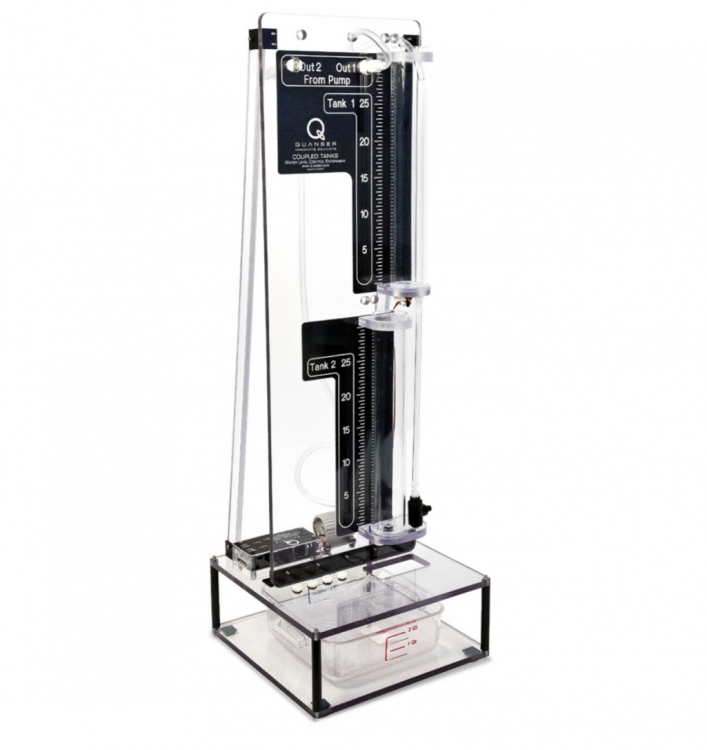
\includegraphics[scale=0.40]{./imagens/tanque-agua.jpg}
	\caption{Tanque Quanser}
\end{figure}

No sistema mostrado a bomba eleva o líquido do reservatório (que está na parte mais baixa), até duas conexões hidráulicas. Tubos podem ser conectados a essas conexões, de modo que ele pode fluir para um dos dois tanques. A partir do tanque 1 o líquido pode passar para o tanque 2, e do tanque 2 pode passar para o reservatório. Cada um dos tanques está equipado com um sensor de nível, que fornece um sinal elétrico em função da altura da coluna do fluido. Esse sistema de tanques acoplados também contém conexões elétricas de entrada e saída, e é possível usa-las para enviar sinais nos sensores, variando entre 0 e 4.8 Volts, para o sistema de aquisição de dados e -12 a 12 Volts para o acionamento da bomba. Três configurações são possíveis:

\begin{figure}[h]
	\centering
	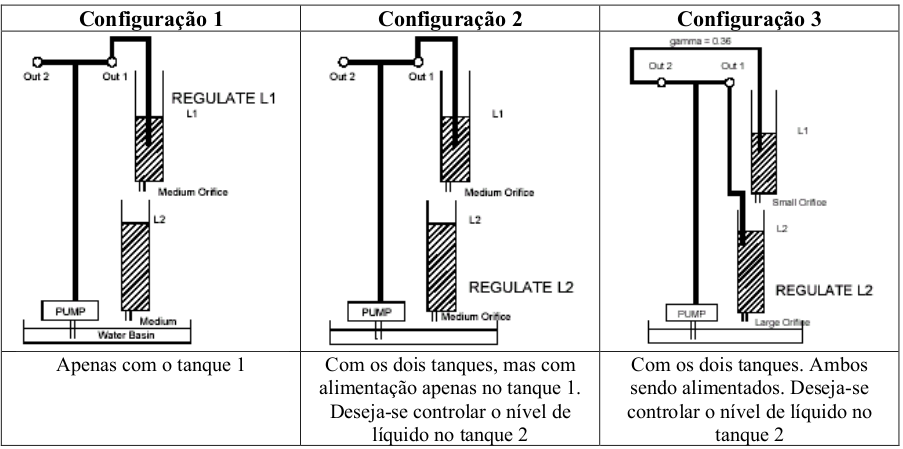
\includegraphics[scale=0.40]{./imagens/configuracoes-tanque.png}
	\caption{Configurações do tanque}
\end{figure}

\end{flushleft}

\pagebreak

%%%%%%%%%% REFERENCIAL TEÓRICO %%%%%%%

\thispagestyle{main}
\section{REFERENCIAL TEÓRICO}



Trata-se da apresentação do embasamento teórico sobre o qual se fundamentará
o trabalho, ou seja, são os pressupostos que darão suporte à abordagem do trabalho.
Lembrar de sempre que utilizar texto de outros lugares, utilizar citação da fonte, como por exemplo, \cite{LATEX04}.

\subsection{Seções}

\subsubsection{Subseções}

\newpage

%%%%%%%%%% METODOLOGIA %%%%%%%%%%%%%%%

\thispagestyle{main}

\section{METODOLOGIA}


\hspace{4ex}A metodologia é caracterizada pela explicação minuciosa dos procedimentos
técnicos realizados durante todo o trabalho.

\subsection{Seções}

\subsubsection{Subseções}

\newpage

%%%%%%%%%% RESULTADOS %%%%%%%%%%%%%%%

\thispagestyle{main}

\section{RESULTADOS}
\hspace{4ex}Como foi dito anteriormente, decidimos usar o modelo de simulação disponibilizado no SIGAA. 

\section{Teste de tensão versus altura da coluna de água}

Usando o MatLab, tentamos determinar, aproximadamente, qual o nível em que os tanques estabilizariam para as tensões determinadas, os valores encontrados são:

\begin{table}[h]
	\centering
	\begin{tabular}{cc}
	\textbf{Tensão de Entrada (V)} & \textbf{Valores de resposta (cm)} \\
	1.0	& ~3 \\
	1.5	& ~6\\
	2.0	& ~11\\
	2.5	& ~25\\
	3.5 & ~18\\
	3.5	& ~35\\
	4.0 & ~45\\
		\multicolumn{1}{l}{} & \multicolumn{1}{l}{} \\
		\multicolumn{1}{l}{} & \multicolumn{1}{l}{}
	\end{tabular}
	\caption{Tensão por altura da coluna de água}
	\label{tab:my-table}
\end{table}

\begin{figure}[H]
	\centering
	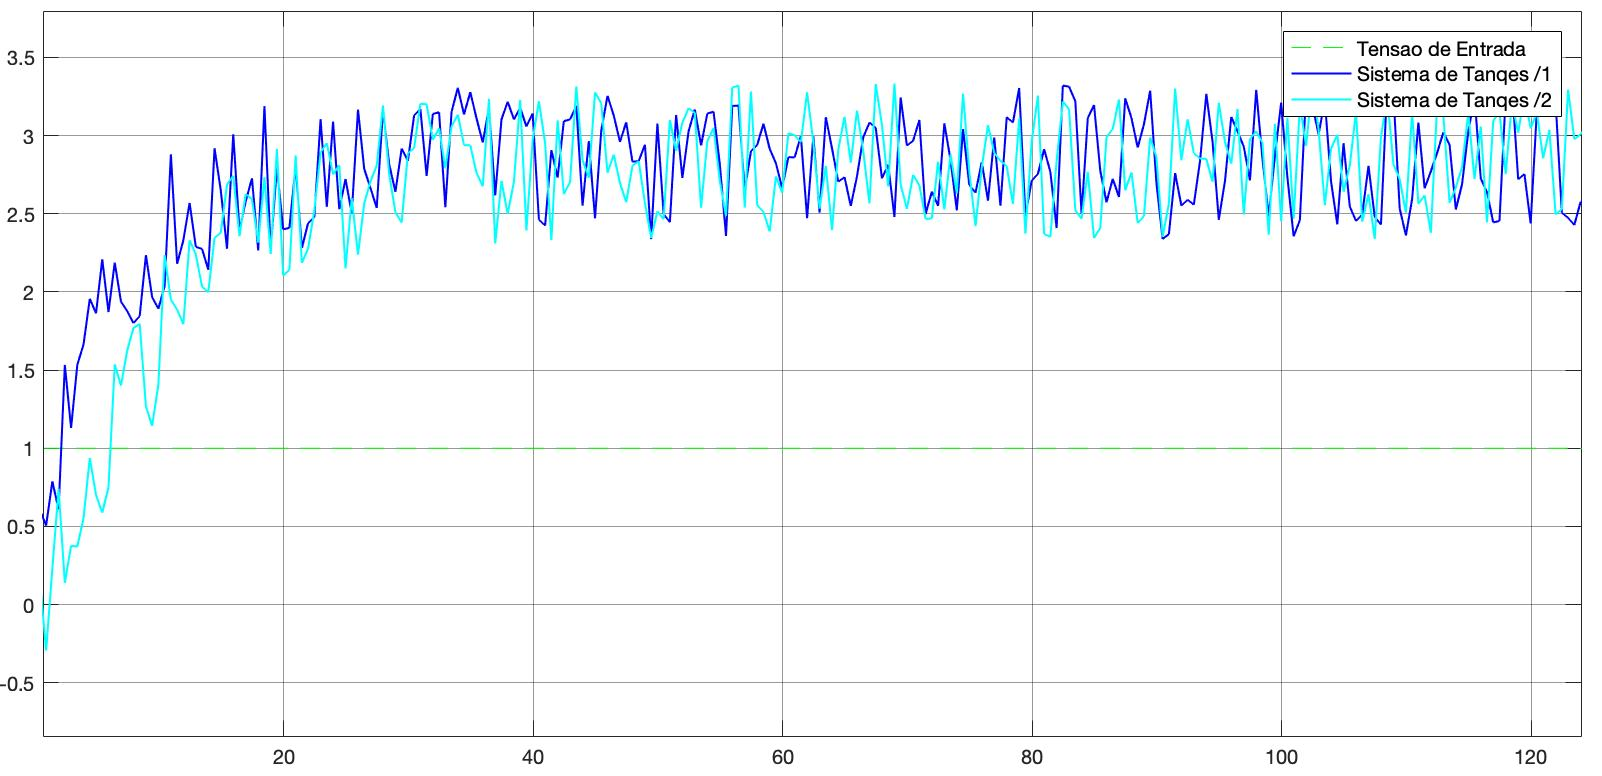
\includegraphics[scale=0.20]{./imagens/exp1/V10.jpg}
	\caption{1.0V e 3cm }
\end{figure}

\begin{figure}[H]
	\centering
	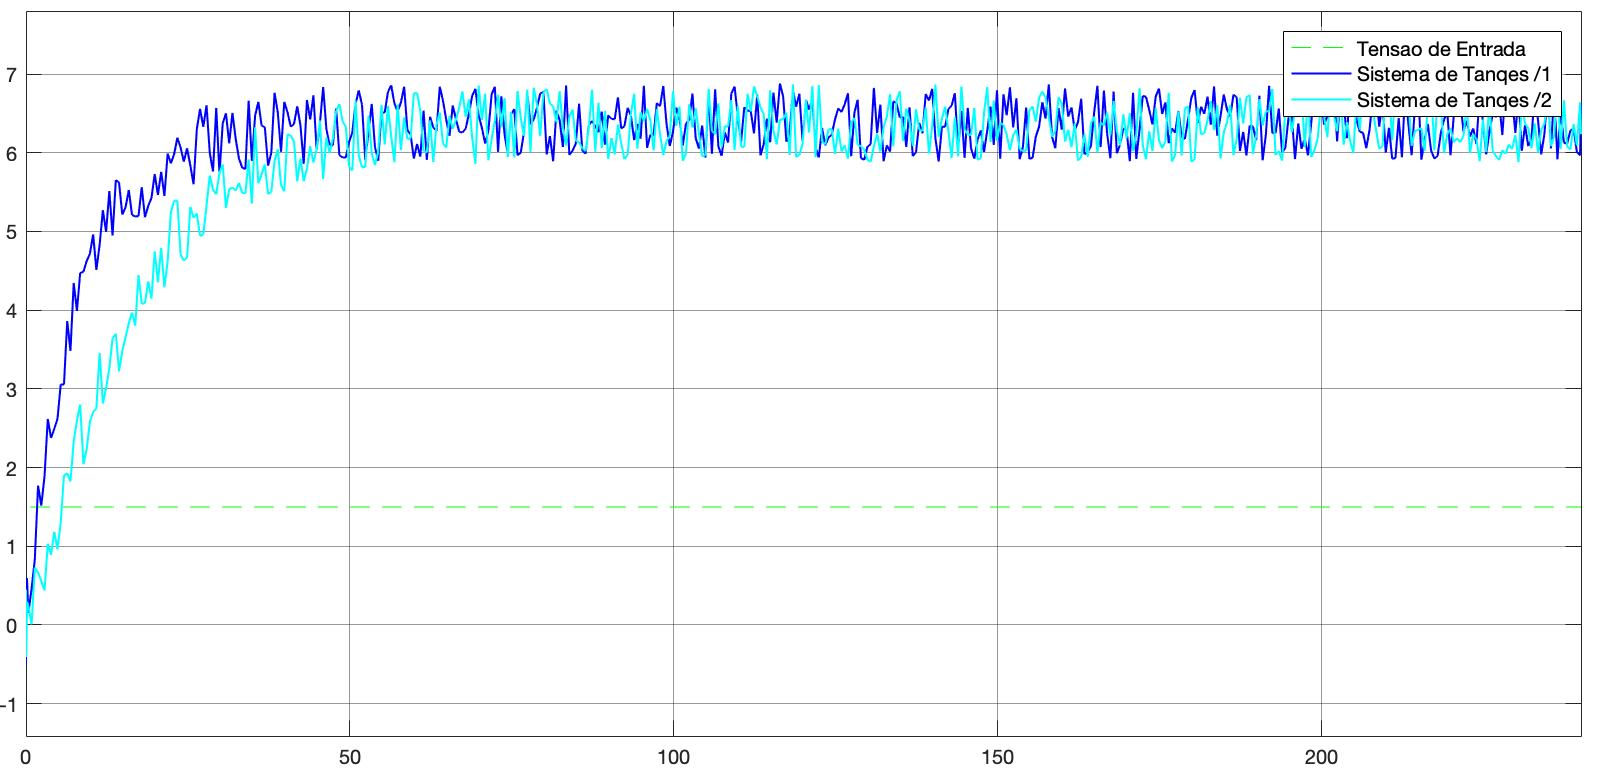
\includegraphics[scale=0.20]{./imagens/exp1/V15.jpg}
	\caption{1.5V e 6cm }
\end{figure}

\begin{figure}[H]
	\centering
	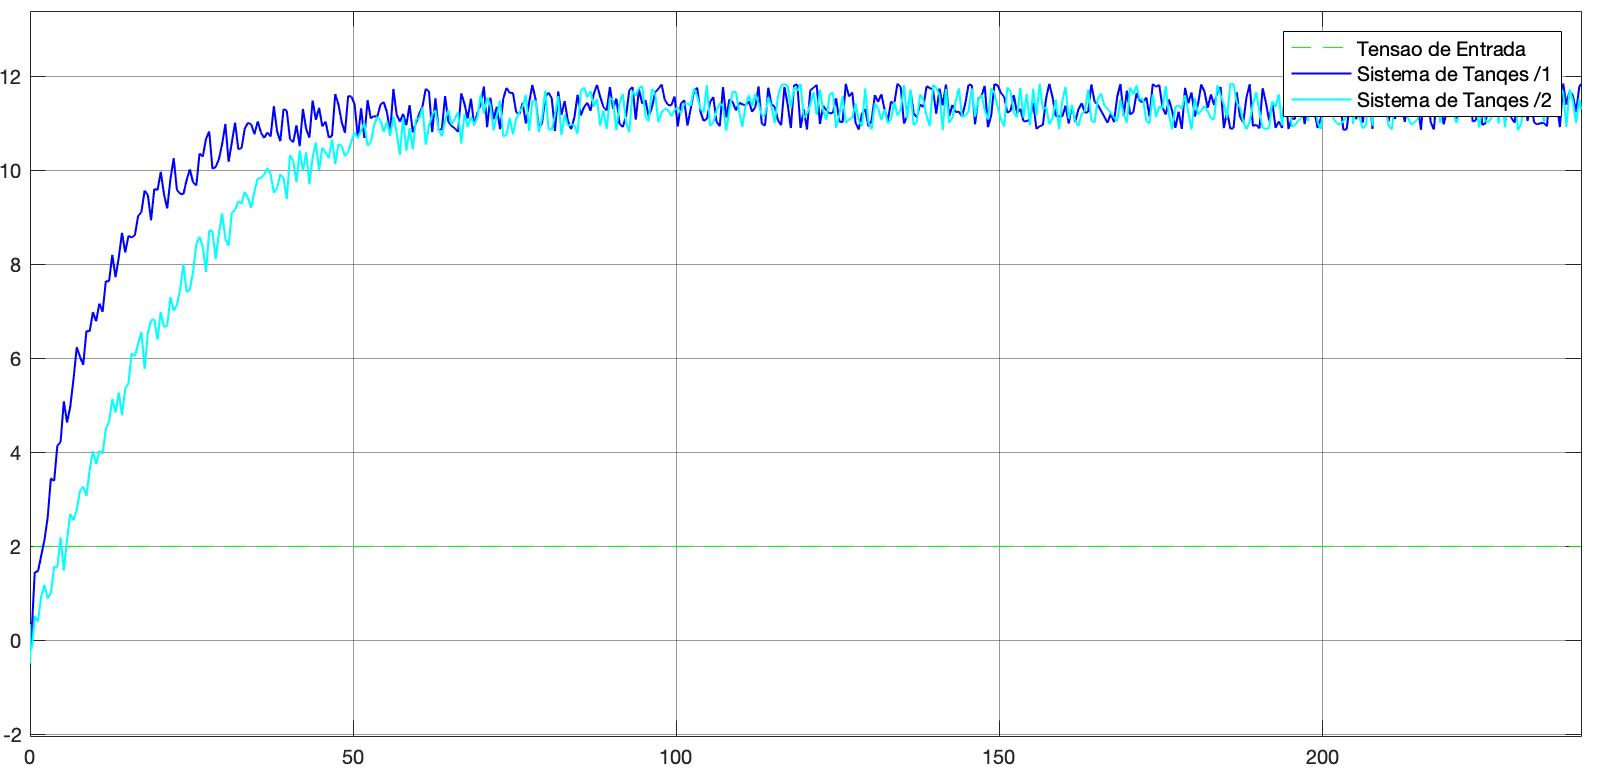
\includegraphics[scale=0.20]{./imagens/exp1/V20.jpg}
	\caption{2.0V e 11cm }
\end{figure}

\begin{figure}[H]
	\centering
	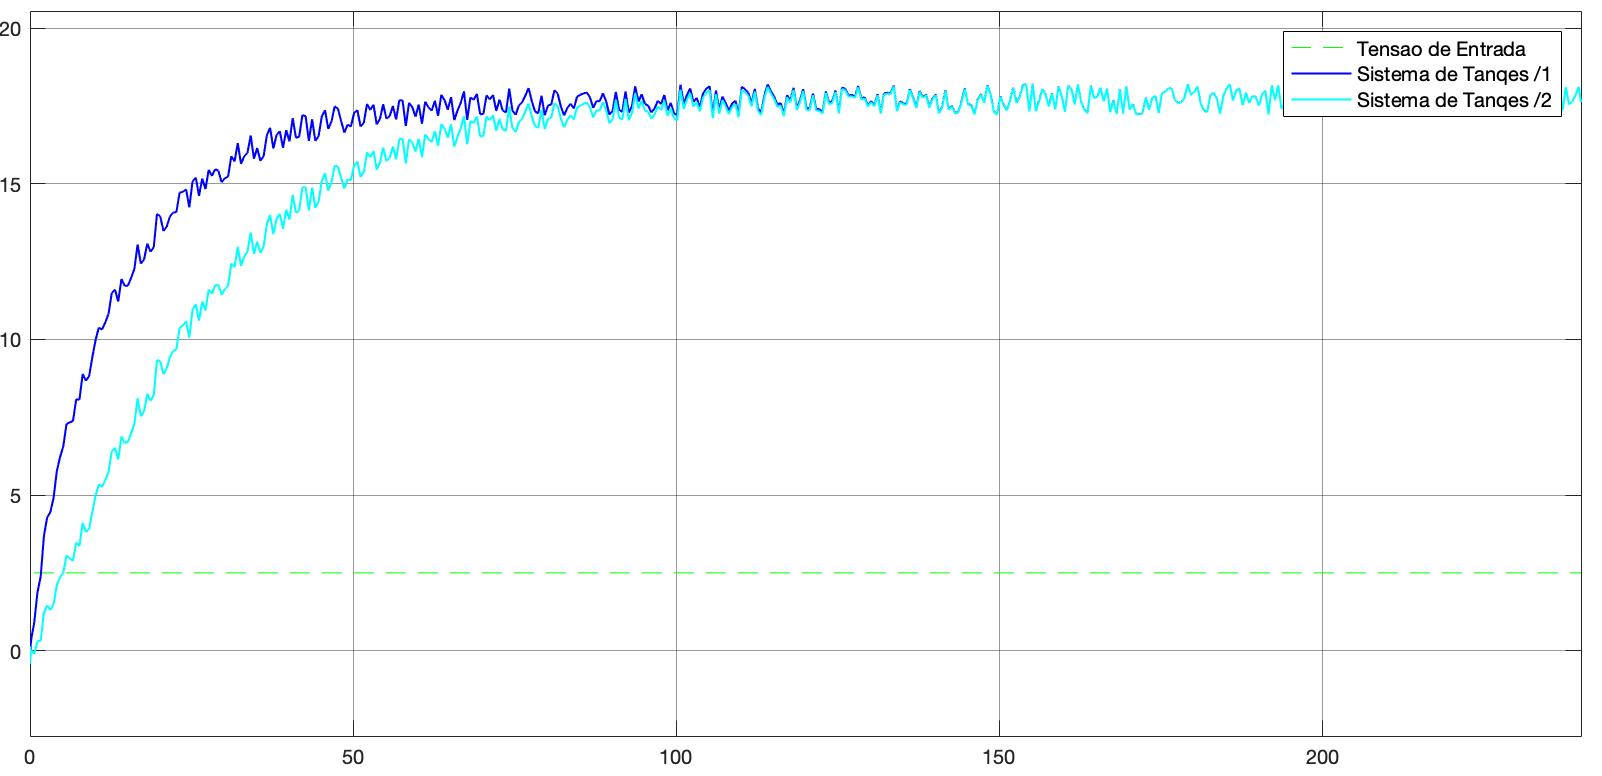
\includegraphics[scale=0.20]{./imagens/exp1/V25.jpg}
	\caption{2.5V e 25cm }
\end{figure}

\begin{figure}[H]
	\centering
	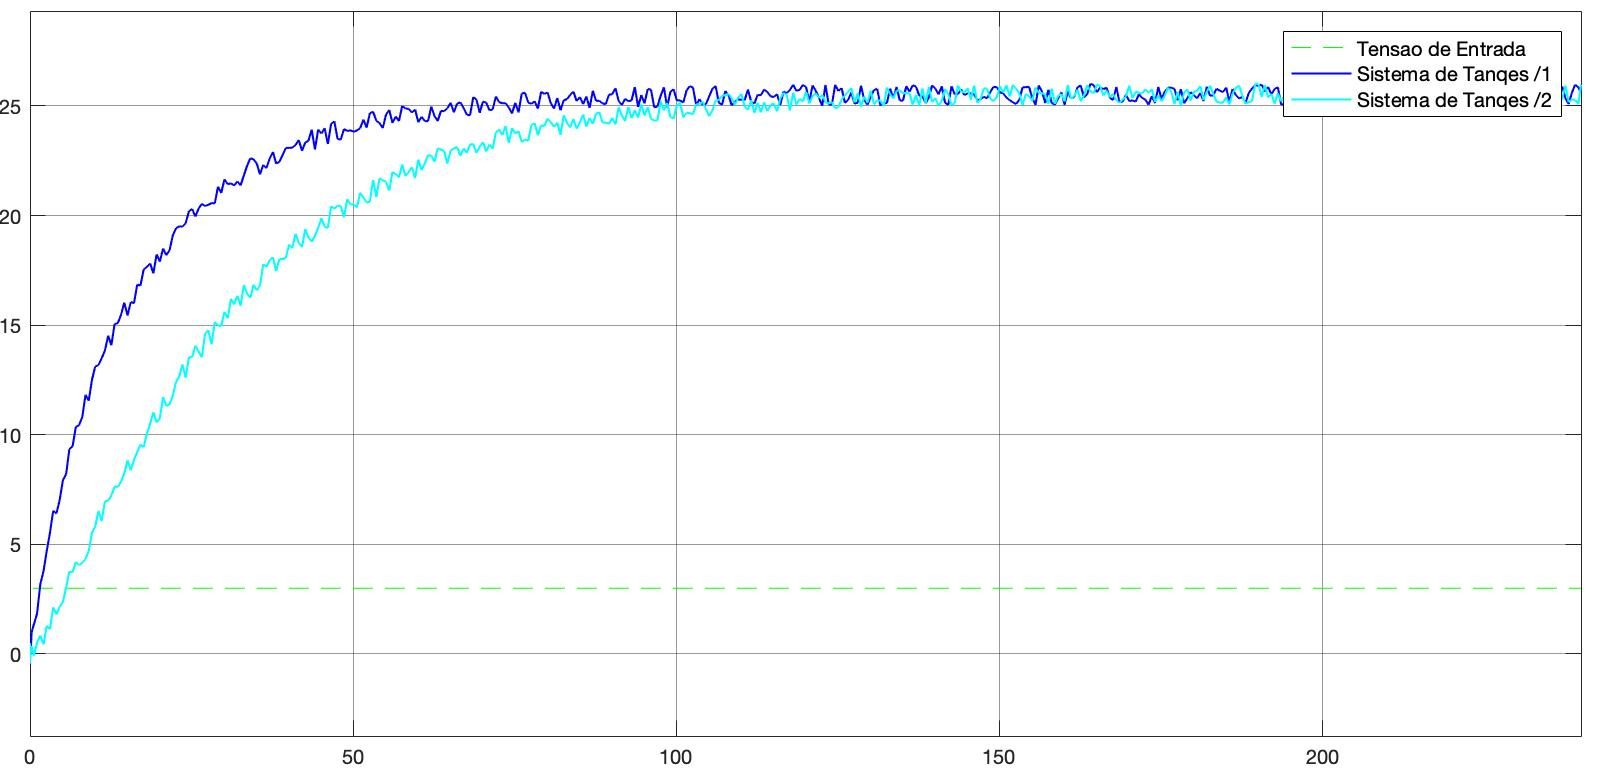
\includegraphics[scale=0.20]{./imagens/exp1/V30.jpg}
	\caption{3.0V e 18cm }
\end{figure}

\begin{figure}[H]
	\centering
	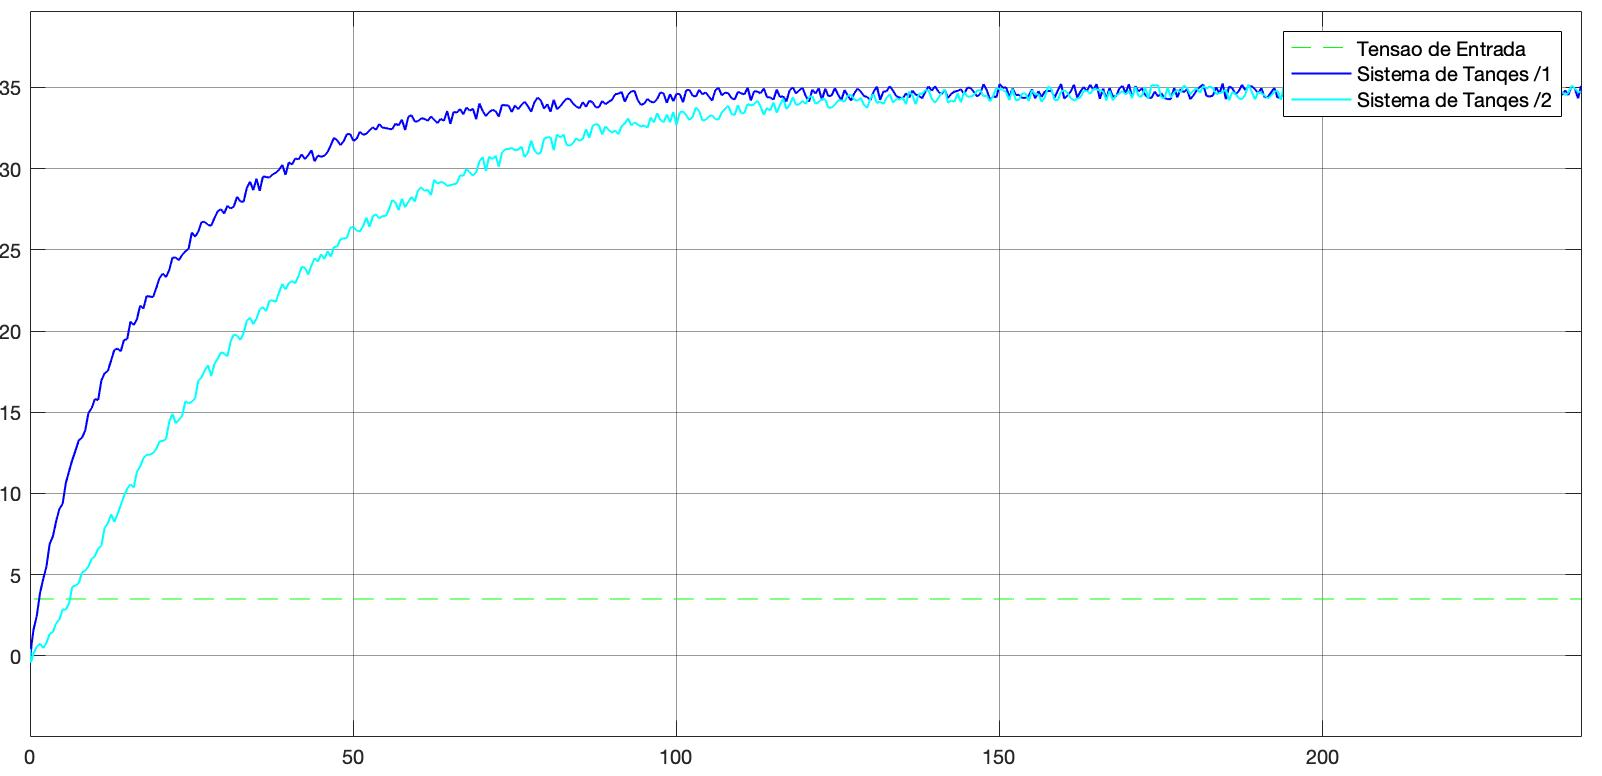
\includegraphics[scale=0.20]{./imagens/exp1/V35.jpg}
	\caption{3.5V e 35cm }
\end{figure}

\begin{figure}[H]
	\centering
	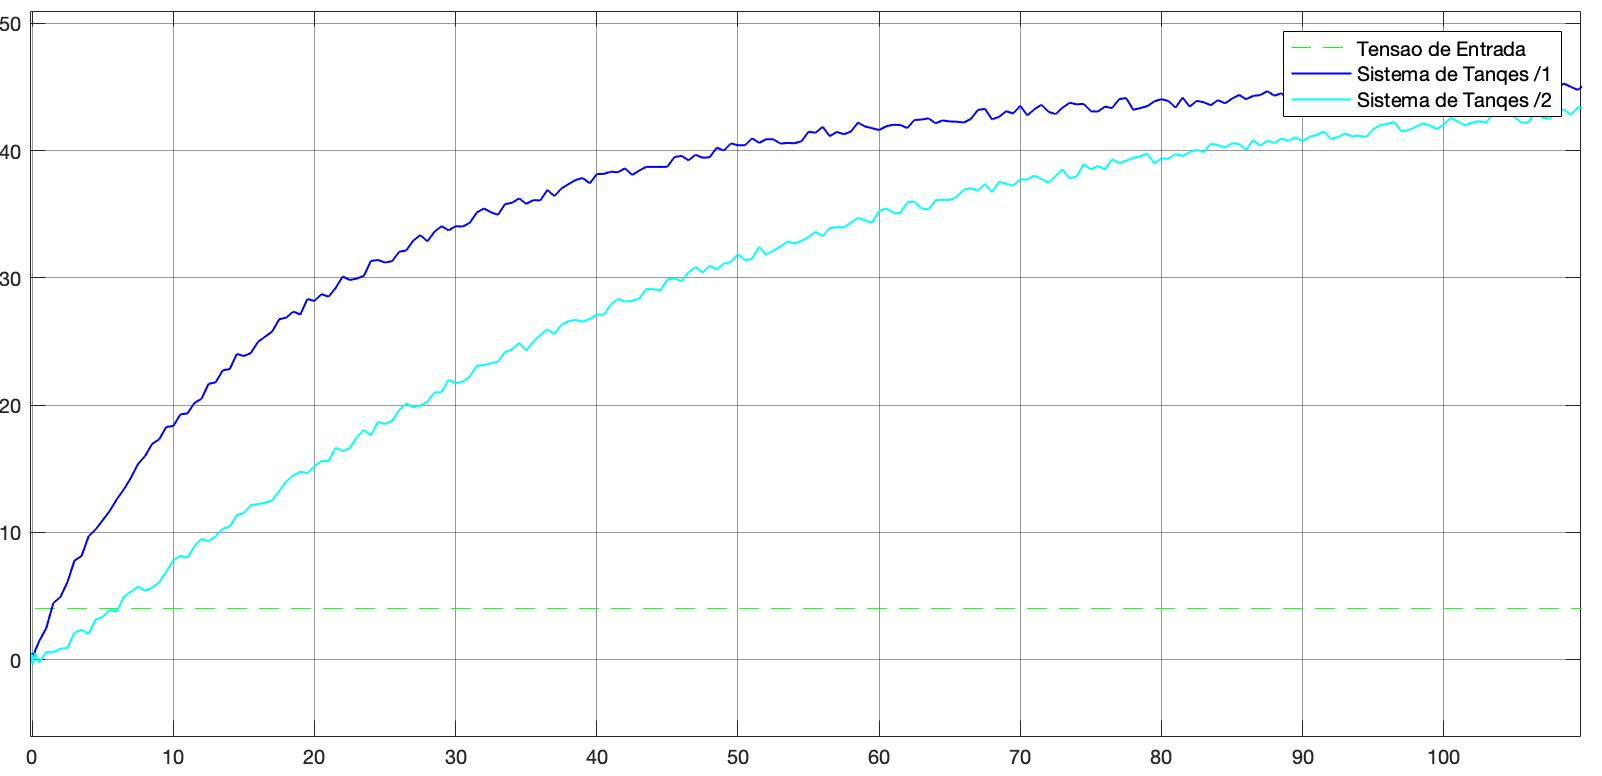
\includegraphics[scale=0.20]{./imagens/exp1/V40.jpg}
	\caption{4.0V e 45cm }
\end{figure}

\section{Teste de coluna de água versus tensão de entrada}
Usando o MatLab, tentamos determinar, aproximadamente, qual o nível em que os tanques estabilizariam para as tensões determinadas, os valores encontrados são:

\begin{table}[h]
	\centering
	\begin{tabular}{cc}
		\textbf{Tensão de Entrada (V)} & \textbf{Valores de resposta (cm)} \\
		~1.0 & 3 \\
		~1.85 & 10\\
		~2.3 & 15\\
		~2.65 & 20\\
		~3.0 & 25\\
		~3.3 & 30\\
		~4.5 & 35\\
		\multicolumn{1}{l}{} & \multicolumn{1}{l}{} \\
		\multicolumn{1}{l}{} & \multicolumn{1}{l}{}
	\end{tabular}
	\caption{Altura da coluna de água em função da tensão}
	\label{tab:my-table2}
\end{table}


\begin{figure}[H]
	\centering
	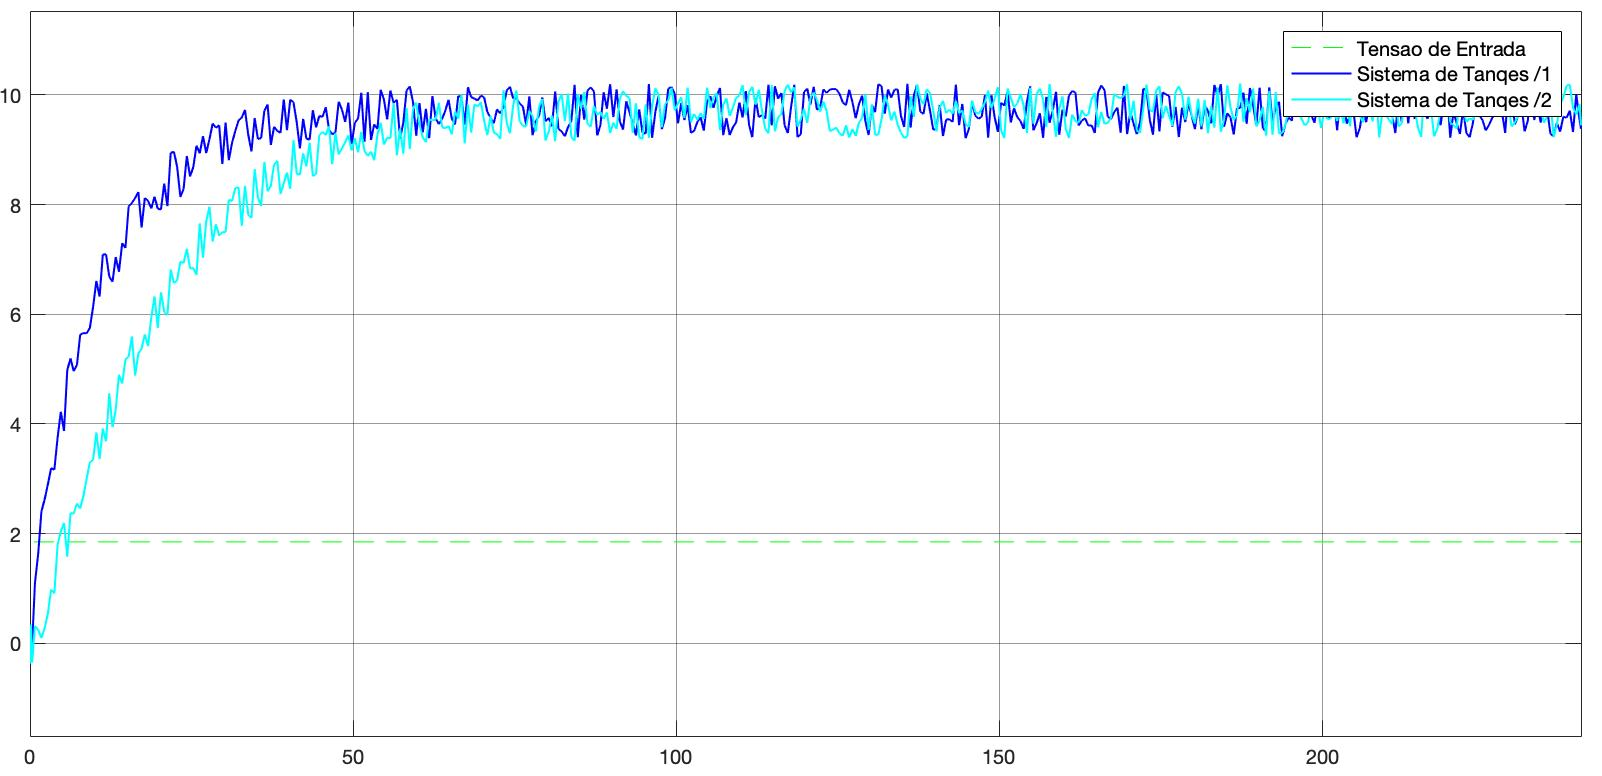
\includegraphics[scale=0.20]{./imagens/exp2/L10.jpg}
	\caption{10cm e 1.85V }
\end{figure}

\begin{figure}[H]
	\centering
	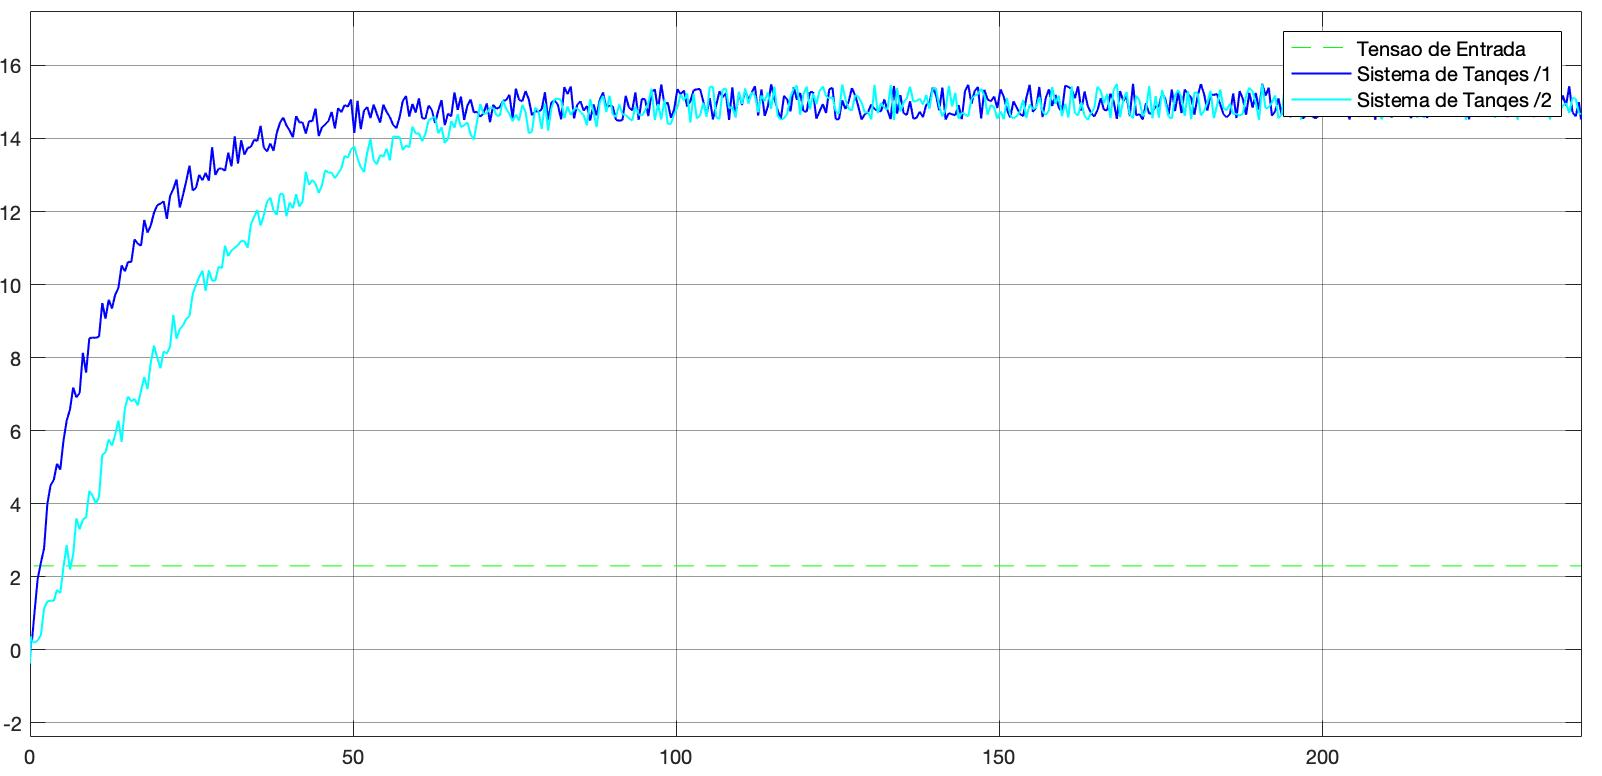
\includegraphics[scale=0.20]{./imagens/exp2/L15.jpg}
	\caption{15cm e 2.3V}
\end{figure}

\begin{figure}[H]
	\centering
	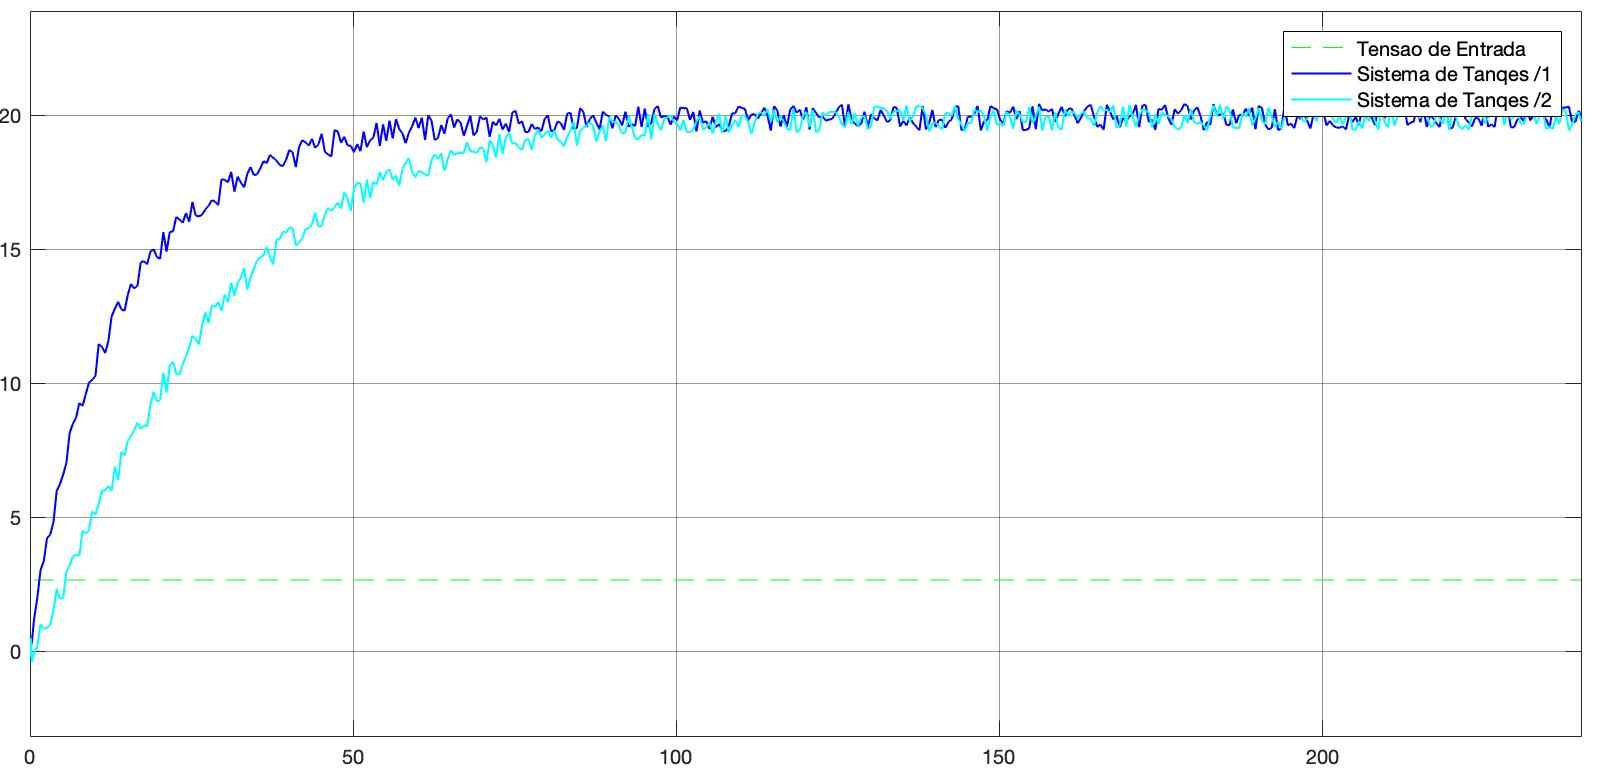
\includegraphics[scale=0.20]{./imagens/exp2/L20.jpg}
	\caption{20cm e 2.65V}
\end{figure}

\begin{figure}[H]
	\centering
	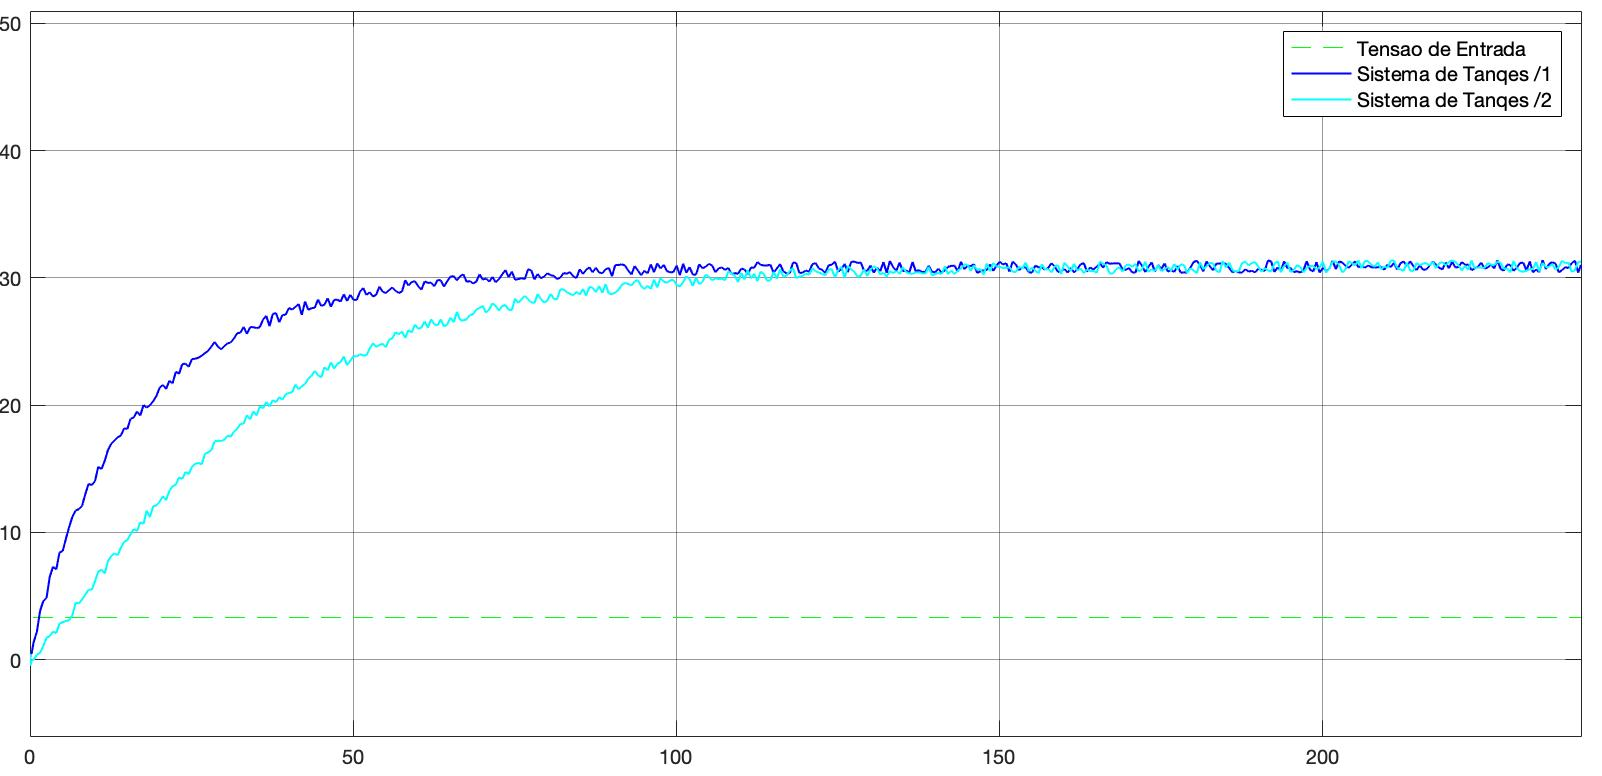
\includegraphics[scale=0.20]{./imagens/exp2/L30.jpg}
	\caption{30cm e 3.3V}
\end{figure}

\pagebreak
\newpage

%%%%%%%%%% CONCLUSÃO %%%%%%%%%%%%%%%

\thispagestyle{main}

\section{CONCLUSÃO}

\hspace{4ex}A conclusão, além de guardar uma proporção relativa ao tamanho do trabalho,
deve guardar uma proporcionalidade também quanto ao conteúdo. Não deve conter
assuntos desnecessários, nem exageros numa linguagem excessivamente técnica e
rebuscada. A conclusão deve dar respostas às questões do trabalho, correspondente aos
objetivos propostos. Deve ser breve, podendo, se necessário, apresentar sugestões para
pesquisas futuras.
\newpage

%%%%%%%% REFERÊNCIAS %%%%%%%%%%%%%%%%%

% Referências bibliogáficas (geradas automaticamente)
\addcontentsline{toc}{chapter}{Referências bibliográficas}
\bibliography{bib/bibliografia}

\appendix

%Apêndice A
\include{apendice}

\end{document}